\documentclass[8pt,a4paper,compress]{beamer}

\usepackage{/home/siyer/lib/slides}

\title{Undirected Graphs}
\date{}
\begin{document}
\begin{frame}
\vfill
\titlepage
\end{frame}

\begin{frame}
\frametitle{Outline}
\tableofcontents
\end{frame}

\section{What are Graphs?}
\begin{frame}[fragile]
\pause

A graph is a set of $V$ vertices connected pairwise by $E$ edges

\smallskip

\begin{center}
\visible<2->{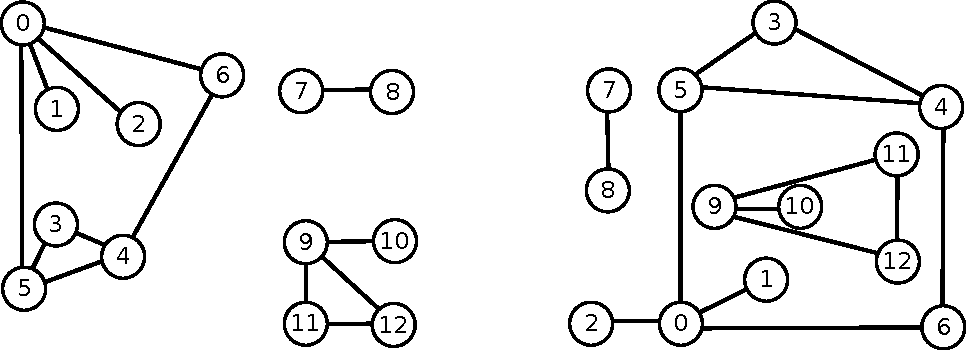
\includegraphics[scale=0.45]{{./figures/graph1}.pdf}}
\end{center}

\pause
\bigskip

We use the names 0 through $V-1$ for the vertices in a $V$-vertex graph

\pause
\bigskip

We use the notation $v$-$w$ to refer to an edge that connects vertices $v$ and $w$

\pause
\bigskip

A self-loop is an edge that connects a vertex to itself

\pause
\bigskip

Parallel edges are edges that connect the same pair of vertices  
\end{frame}

\begin{frame}[fragile]
\begin{minipage}{200pt}
\pause

The degree of a vertex is the number of vertices connected to it

\pause
\bigskip

A path is a sequence of vertices connected by edges

\pause
\bigskip

A cycle is a path with at least one edge whose first and last vertices are the same

\pause
\bigskip

The length of a path or a cycle is its number of edges

\pause
\bigskip

A graph is connected if there is a path from every vertex to every other vertex in the graph

\pause
\bigskip

A graph that is not connected consists of a set of connected components, which are maximal connected subgraphs
\end{minipage}%
\begin{minipage}{100pt}
\begin{center}
\visible<2->{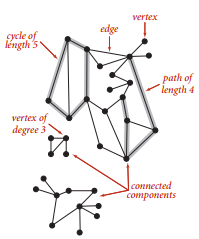
\includegraphics[scale=0.4]{{./figures/graph2}.pdf}}
\end{center}
\end{minipage}
\end{frame}

\begin{frame}[fragile]
\begin{minipage}{200pt}
\pause

An acyclic graph is a graph with no cycles

\pause
\bigskip

A tree is an acyclic connected graph

\pause
\bigskip

A bipartite graph is a graph whose vertices can be divided into two sets such that all edges connect a vertex in one set with a vertex in the other set
\end{minipage}%
\begin{minipage}{100pt}
\begin{center}
\visible<2->{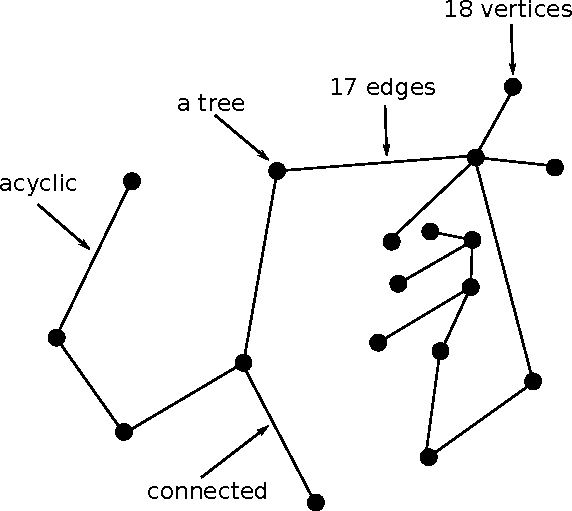
\includegraphics[scale=0.4]{{./figures/graph3}.pdf}}

\bigskip

\visible<2->{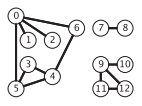
\includegraphics[scale=0.4]{{./figures/graph4}.pdf}}
\end{center}
\end{minipage}
\end{frame}

\begin{frame}[fragile]
\pause

Graph applications
\begin{center}
\begin{tabular}{ccc}
graph & vertex & edge \\ \hline
communication & telephone, computer & fiber optic cable \\
circuit & gate, register, processor & wire \\
mechanical & joint & rod, beam, spring \\
financial & stock, currency & transactions \\
transportation & intersection & street \\
internet & class C network & connection \\
game & board position & legal move \\
social relationship & person & friendship \\
neural network & neuron & synapse \\
protein network & protein & protein-protein interaction \\
molecule & atom & bond
\end{tabular}  
\end{center}
\end{frame}

\begin{frame}[fragile]
\pause

Example: Internet graph

\smallskip

\begin{center}
\visible<2->{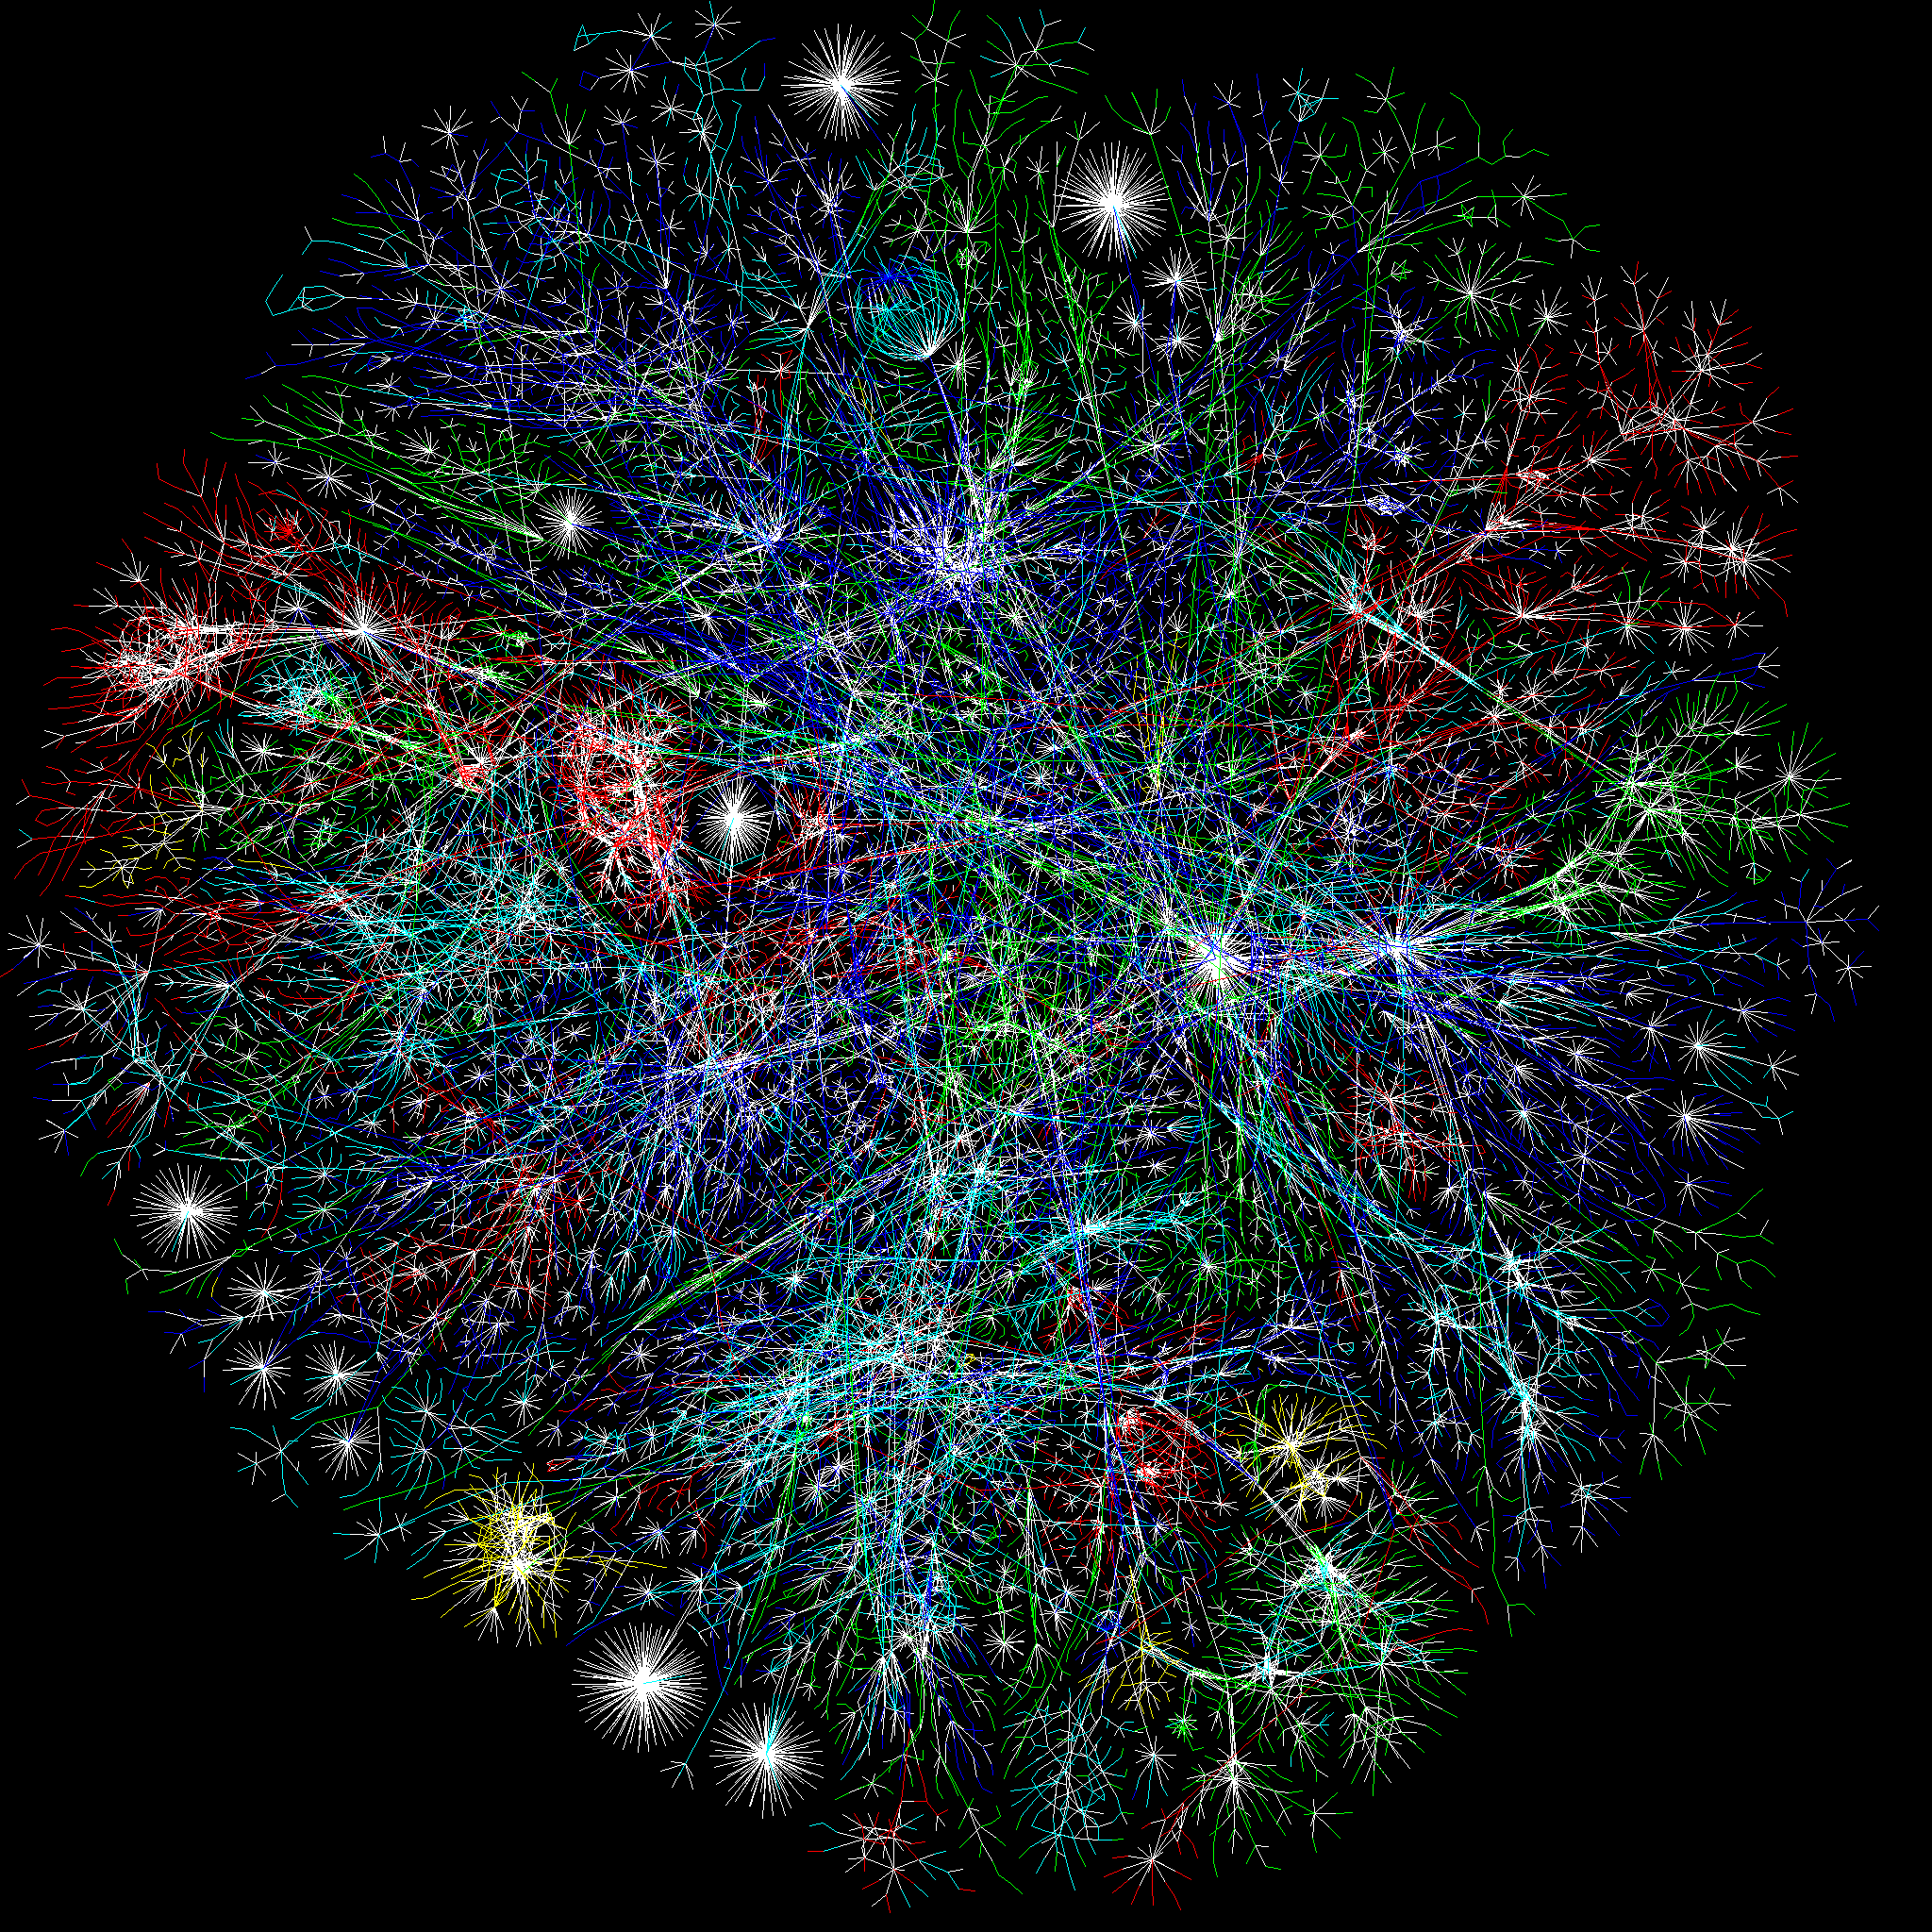
\includegraphics[scale=0.1]{{./figures/internet}.png}}
\end{center}
\end{frame}

\begin{frame}[fragile]
\pause

Example: facebook graph

\smallskip

\begin{center}
\visible<2->{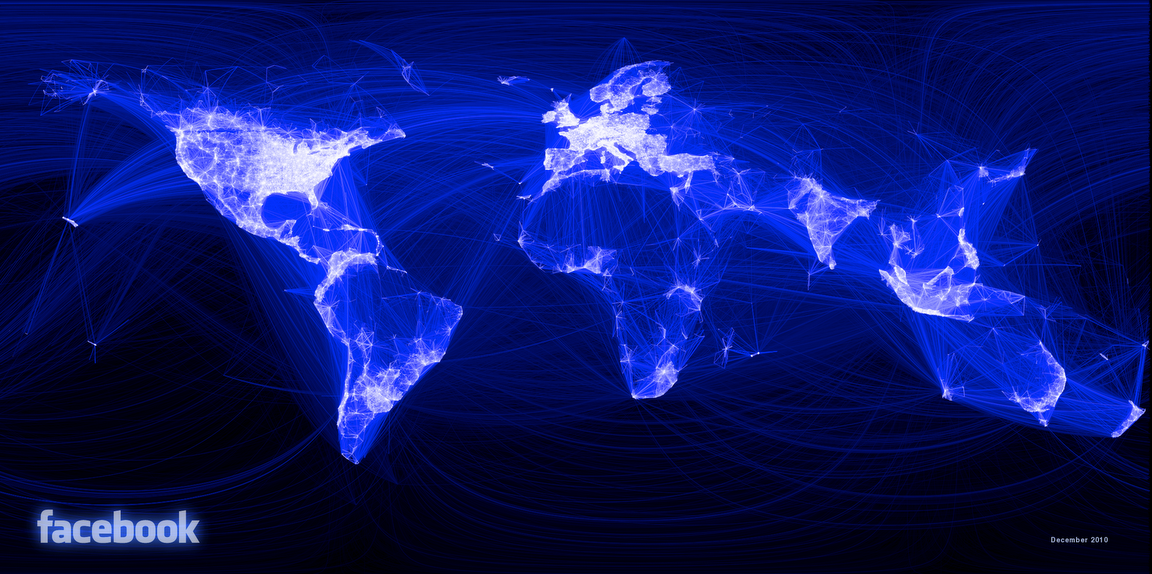
\includegraphics[scale=0.25]{{./figures/facebook}.png}}
\end{center}
\end{frame}

\begin{frame}[fragile]
\pause

Example: c.elegans connectome graph

\smallskip

\begin{center}
\visible<2->{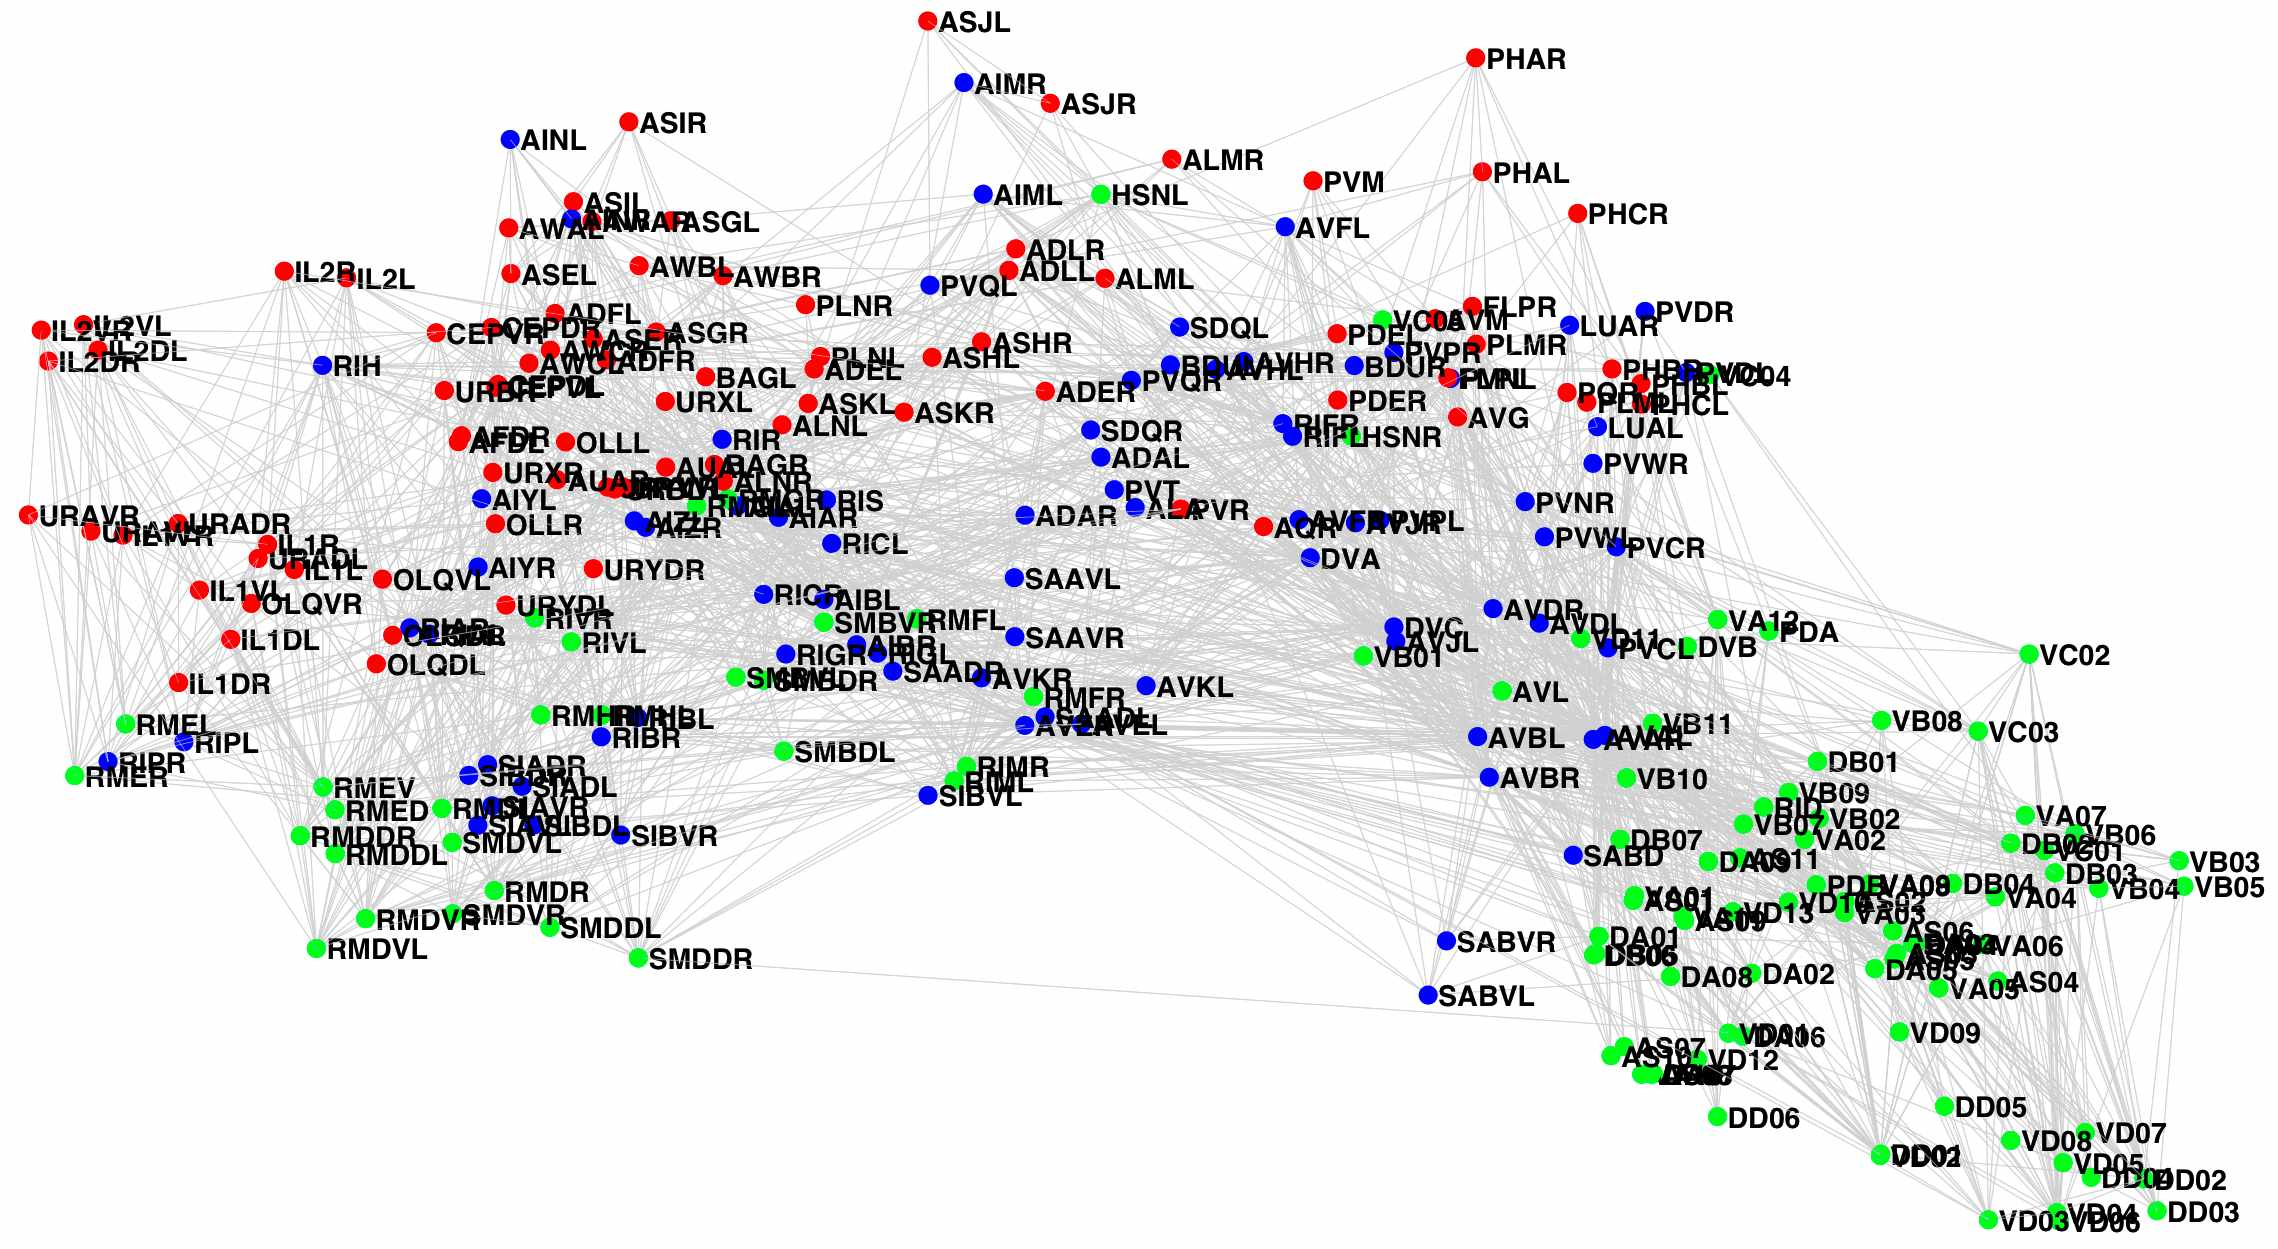
\includegraphics[scale=0.12]{{./figures/celegans}.png}}
\end{center}
\end{frame}

\begin{frame}[fragile]
\pause

Example: coauthorship graph

\smallskip

\begin{center}
\visible<2->{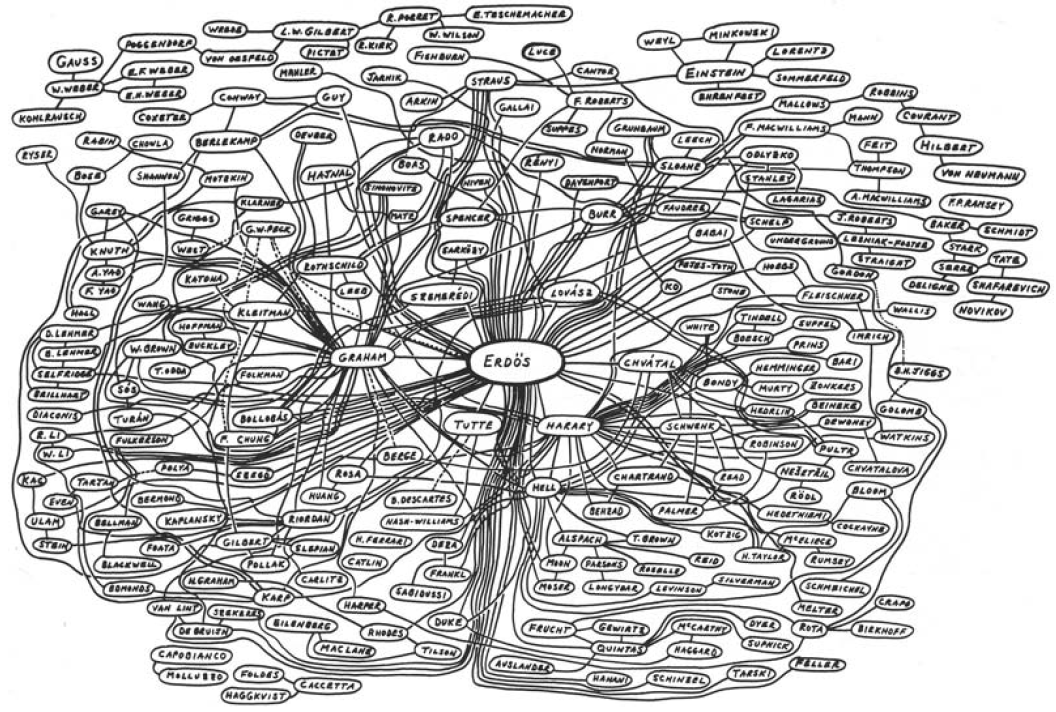
\includegraphics[scale=0.25]{{./figures/erdos}.png}}
\end{center}
\end{frame}

\begin{frame}[fragile]
\pause

Some graph-processing problems
\begin{center}
\begin{tabular}{cc}
problem & description \\ \hline
$s$-$t$ path & is there a path between $s$ and $t$? \\ 
shortest $s$-$t$ path & what is the shortest path between $s$ and $t$? \\
cycle & is there a cycle in the graph? \\
Euler cycle & is there a cycle that uses each edge exactly once? \\
Hamilton cycle & is there a cycle that uses each vertex exactly once? \\
connectivity & is there a way to connect all of the vertices? \\
biconnectivity & is there a vertex whose removal disconnects the graph? \\
bipartiteness & is a graph bipartite? \\ 
planarity & can the graph be drawn in the plane with no crossing edges? \\
graph isomorphism & do two graph representations denote the same graph?
\end{tabular}  
\end{center}
\end{frame}

\section{Undirected Graphs}
\begin{frame}[fragile]
\pause

Undirected graph API
\begin{center}
\begin{tabular}{cc}
method & description \\ \hline
\lstinline$Graph(int V)$ & create a $V$-vertex graph with no edges \\ 
\lstinline$Graph(In in)$ & read a graph from input stream $in$ \\
\lstinline$int V()$      & number of vertices \\
\lstinline$int E()$      & number of edges \\
\lstinline$void addEdge(int v, int w)$ & add edge $v$-$w$ to this graph \\
\lstinline$Iterable<Integer> adj(int v)$ & vertices adjacent to $v$
\end{tabular} 
\end{center}

\pause

Graph input format
\begin{minipage}{150pt}
\begin{lstlisting}[language={}]
$ more tinyG.txt
13 13 
0 5 4 3 0 1 9 12 6 4 5 4 0 2 
11 12 9 10 0 6 7 8 9 11 5 3
\end{lstlisting}
\end{minipage}%
\begin{minipage}{150pt}
\begin{center}
\visible<3->{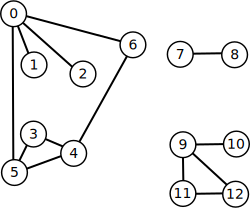
\includegraphics[scale=0.4]{{./figures/graph5}.pdf}}
\end{center}
\end{minipage}

\pause
\bigskip

Typical graph-processing code
\begin{lstlisting}[language=Java]
public static int degree(Graph G, int v) {
    int degree = 0;
    for (int w : G.adj(v)) { 
        degree++; 
    }
    return degree;
}
\end{lstlisting}
\end{frame}

\begin{frame}[fragile]
\pause

Graph representations
\begin{itemize}
\item Edge list: maintain a list of the edges (linked list or array)

\item Adjacency matrix: maintain a $V$-by-$V$ matrix $M$, such that $M[v][w]$ is 1 if there is an edge from $v$ to $w$, and 0 otherwise

\item Adjacency list: maintain a vertex-indexed array of lists
\end{itemize}

\pause
\bigskip

Performance characteristics
\begin{center}
\begin{tabular}{ccccc}
representation & space & add edge & is $v$-$w$ an edge? & enumerate \lstinline$adj(v)$ \\ \hline
edge list & $E$ & 1 & $E$ & $E$ \\
adjacency matrix & $V^2$ & 1$^\dagger$ & 1 & $V$ \\ 
adjacency list & $E+V$ & 1 & $degree(v)$ & $degree(v)$ 
\end{tabular}  

\smallskip

\small $\dagger$ disallows parallel edges
\end{center}
\end{frame}

\begin{frame}[fragile]
\pause

Implementation of \lstinline{Graph} data type using an adjacency list
\begin{lstlisting}[language=Java]
package edu.princeton.cs.algs4;

public class Graph {
    private final int V;
    private int E;
    private LinkedBag<Integer>[] adj;

    public Graph(int V) {
        if (V < 0) {
            throw new IllegalArgumentException(); 
        }
        this.V = V;
        this.E = 0;
        adj = (LinkedBag<Integer>[]) new LinkedBag[V];
        for (int v = 0; v < V; v++) {
            adj[v] = new LinkedBag<Integer>();
        }
    }

    public Graph(In in) {
        this(in.readInt());
        int E = in.readInt();
        if (E < 0) { 
            throw new IllegalArgumentException();
        }
        for (int i = 0; i < E; i++) {
            int v = in.readInt();
            int w = in.readInt();
            addEdge(v, w);
        }
    }
\end{lstlisting}
\end{frame}

\begin{frame}[fragile]
\pause

\begin{lstlisting}[language=Java]
    public int V() { return V; }

    public int E() { return E; }
 
    private void validateVertex(int v) {
        if (v < 0 || v >= V) {
            throw new IndexOutOfBoundsException();
        }
    }

    public void addEdge(int v, int w) {
        validateVertex(v);
        validateVertex(w);
        E++;
        adj[v].add(w);
        adj[w].add(v);
    }

    public Iterable<Integer> adj(int v) {
        validateVertex(v);
        return adj[v];
    }
}
\end{lstlisting}
\end{frame}

\section{Depth-First Search (DFS)}
\begin{frame}[fragile]
\pause

\begin{minipage}{210pt}
Goal: systematically traverse a graph

\pause
\bigskip

Idea: mimic maze exploration

\pause
\bigskip

Typical applications
\begin{itemize}
\item Find all vertices connected to a given source vertex
\item Find a path between two vertices
\end{itemize}

\pause
\bigskip

To visit a vertex $v$
\begin{itemize}
\item Mark vertex $v$ as visited
\item Recursively visit all unmarked vertices adjacent to $v$
\end{itemize}

\pause
\bigskip

Data structures
\begin{itemize}
\item Boolean array \lstinline{marked[][]} to mark visited vertices
\item Integer array \lstinline{edgeTo[]} to keep track of paths; \lstinline{edgeTo[w] = v} means that edge $v$-$w$ taken to visit $w$ for first time
\end{itemize}
\end{minipage}
\begin{minipage}{90pt}
\begin{center}
\visible<2->{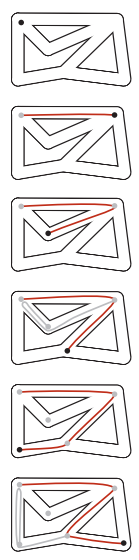
\includegraphics[scale=0.4]{{./figures/dfs_maze}.png}}
\end{center}
\end{minipage}
\end{frame}

\begin{frame}[fragile]
\pause

Design pattern for graph processing: decouple graph data type from graph processing
\begin{itemize}
\item Create a \lstinline{Graph} object
\item Pass the \lstinline{Graph} object to a graph-processing routine
\item Query the graph-processing routine for information
\end{itemize}

\begin{center}
\begin{tabular}{cc}
method & description \\ \hline
\lstinline$Paths(Graph G, int s)$ & find paths in $G$ from source $s$ \\
\lstinline$boolean hasPathTo(int v)$ & is there a path from $s$ to $v$? \\
\lstinline$Iterable<Integer> pathTo(int v)$ & path from $s$ to $v$, or \lstinline$null$
\end{tabular} 
\end{center}

\pause
\bigskip

Typical graph-processing code
\begin{lstlisting}[language=Java]
Paths paths = new Paths(G, s);
for (int v = 0; v < G.V(); v++) {
    if (paths.hasPathTo(v)) {
        StdOut.println(v);
    }
}
\end{lstlisting}
\end{frame}

\begin{frame}[fragile]
\pause

\begin{lstlisting}[language=Java]
package edu.princeton.cs.algs4;

public class DepthFirstPaths {
    private boolean[] marked; 
    private int[] edgeTo; 
    private final int s; 

    public DepthFirstPaths(Graph G, int s) {
        this.s = s;
        edgeTo = new int[G.V()];
        marked = new boolean[G.V()];
        dfs(G, s);
    }

    private void dfs(Graph G, int v) {
        marked[v] = true;
        for (int w : G.adj(v)) {
            if (!marked[w]) {
                edgeTo[w] = v;
                dfs(G, w);
            }
        }
    }

    public boolean hasPathTo(int v) { return marked[v]; }

    public Iterable<Integer> pathTo(int v) {
        if (!hasPathTo(v)) { return null; }
        LinkedStack<Integer> path = new LinkedStack<Integer>();
        for (int x = v; x != s; x = edgeTo[x]) { path.push(x); }
        path.push(s);
        return path;
    }
}
\end{lstlisting}
\end{frame}

\begin{frame}[fragile]
\pause

Trace
\begin{center}
\visible<2->{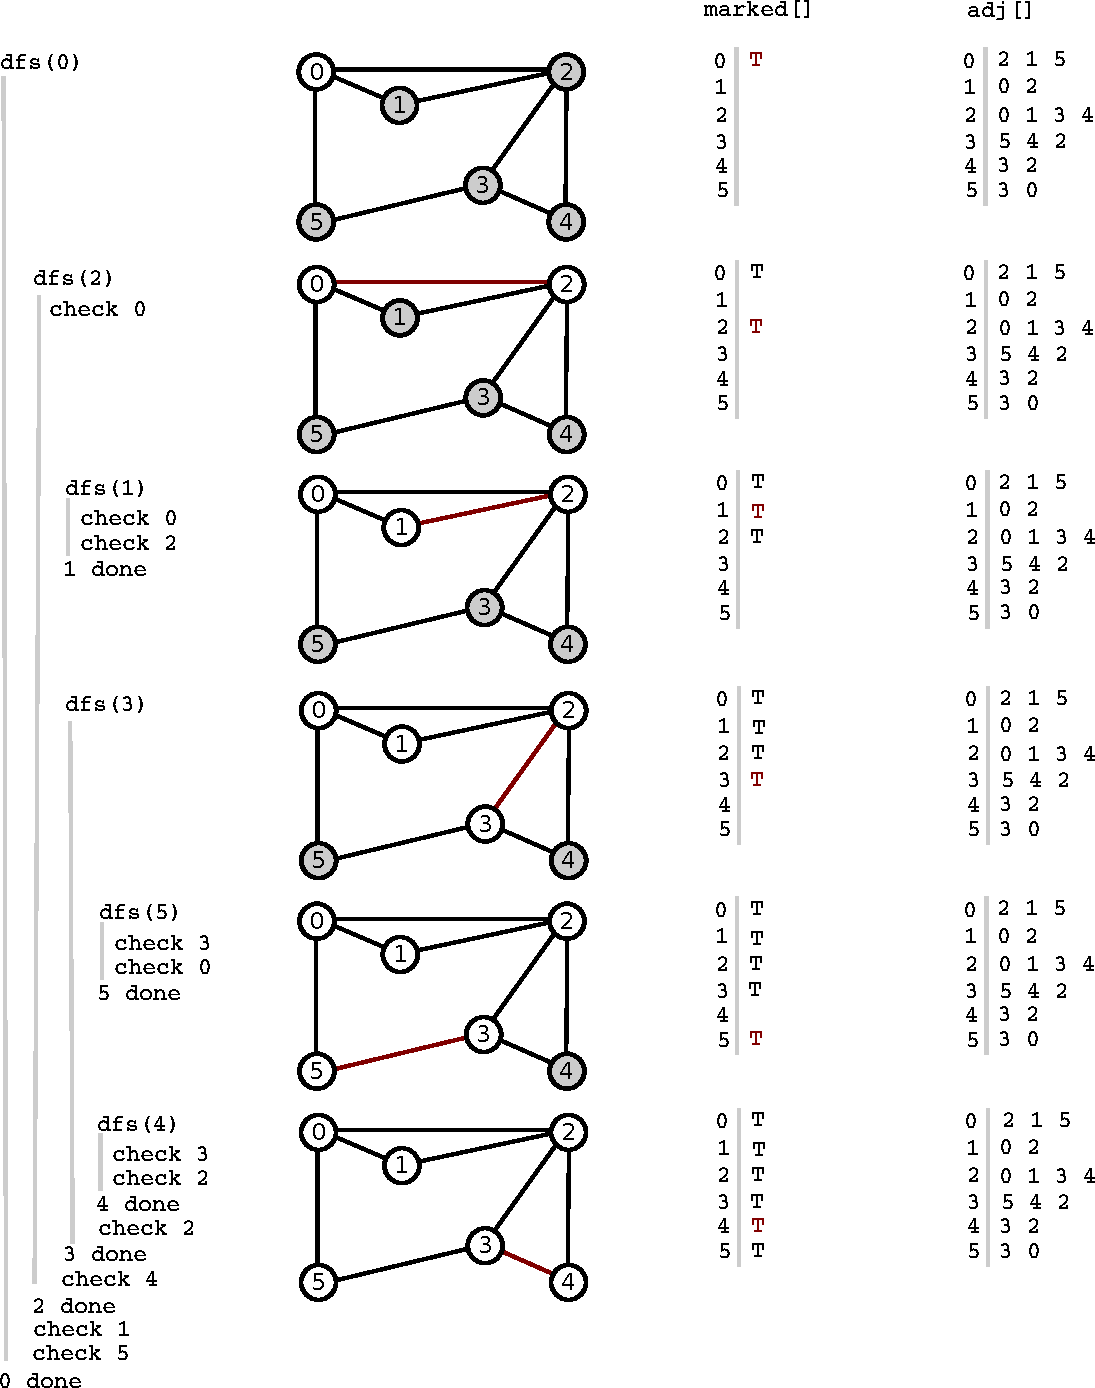
\includegraphics[scale=0.36]{{./figures/dfs_trace}.pdf}}
\end{center}
\end{frame}

\section{Breadth-First Search (BFS)}
\begin{frame}[fragile]
\pause

\begin{minipage}{210pt}
Goal: given a graph and a source vertex $s$, support queries of the form
\begin{itemize}
\item Is there a path from $s$ to a given target vertex $v$?

\item If so, find a shortest such path (one with minimal number of edges)
\end{itemize}

\pause
\bigskip

Repeat until queue is empty
\begin{itemize}
\item Remove vertex $v$ from queue

\item Add to queue all unmarked vertices adjacent to v and mark them
\end{itemize}
\end{minipage}
\begin{minipage}{90pt}
\begin{center}
\visible<2->{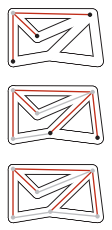
\includegraphics[scale=0.4]{{./figures/bfs_maze}.png}}
\end{center}
\end{minipage}
\end{frame}

\begin{frame}[fragile]
\pause

\begin{lstlisting}[language=Java]
package edu.princeton.cs.algs4;

public class BreadthFirstPaths {
    private static final int INFINITY = Integer.MAX_VALUE;
    private boolean[] marked; 
    private int[] edgeTo; 
    private int[] distTo;   

    public BreadthFirstPaths(Graph G, int s) {
        marked = new boolean[G.V()];
        distTo = new int[G.V()];
        edgeTo = new int[G.V()];
        bfs(G, s);
    }

    private void bfs(Graph G, int s) {
        LinkedQueue<Integer> q = new LinkedQueue<Integer>();
        for (int v = 0; v < G.V(); v++) { distTo[v] = INFINITY; }
        distTo[s] = 0;
        marked[s] = true;
        q.enqueue(s);
        while (!q.isEmpty()) {
            int v = q.dequeue();
            for (int w : G.adj(v)) {
                if (!marked[w]) {
                    edgeTo[w] = v;
                    distTo[w] = distTo[v] + 1;
                    marked[w] = true;
                    q.enqueue(w);
                }
            }
        }
    }
\end{lstlisting}
\end{frame}

\begin{frame}[fragile]
\pause

\begin{lstlisting}[language=Java]
    public boolean hasPathTo(int v) { return marked[v]; }

    public int distTo(int v) { return distTo[v]; }

    public Iterable<Integer> pathTo(int v) {
        if (!hasPathTo(v)) return null;
        LinkedStack<Integer> path = new LinkedStack<Integer>();
        int x;
        for (x = v; distTo[x] != 0; x = edgeTo[x]) {
            path.push(x);
        }
        path.push(x);
        return path;
    }
}
\end{lstlisting}
\end{frame}

\begin{frame}[fragile]
\pause

Trace
\begin{center}
\visible<2->{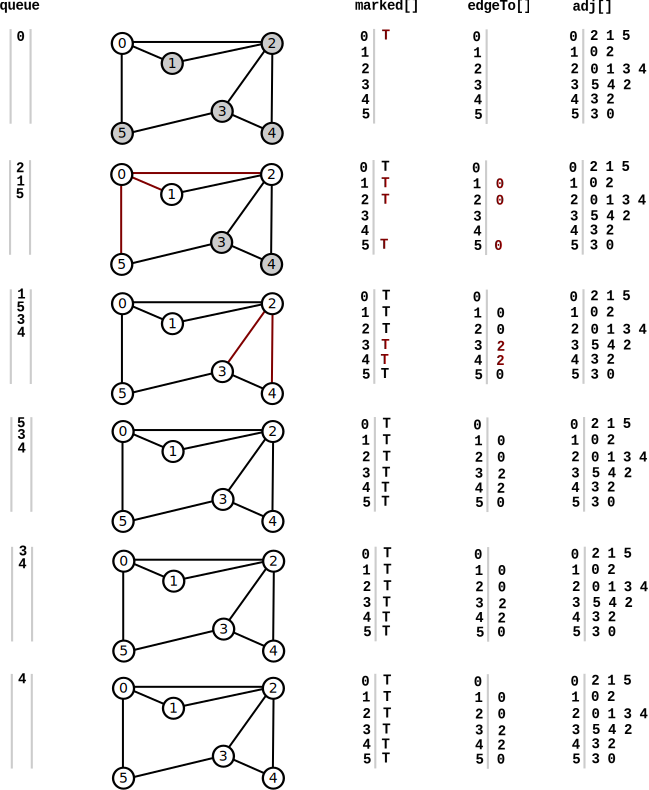
\includegraphics[scale=0.37]{{./figures/bfs_trace}.pdf}}
\end{center}
\end{frame}

\section{Connected Components}
\begin{frame}[fragile]
\pause

Vertices $v$ and $w$ are connected if there is a path between them

\pause
\bigskip

Goal: preprocess graph to answer queries of the form is $v$ connected to $w$ in constant time

\begin{center}
\begin{tabular}{cc}
method & description \\ \hline
\lstinline$CC(Graph G)$ & find connected components in $G$ \\
\lstinline$boolean connected(int v, int w)$ & are $v$ and $w$ connected? \\
\lstinline$int count()$ & number of connected components \\
\lstinline$int id(int v)$ & component identifier for $v$ \\
\lstinline$int size(int v)$ & number of vertices in $v$'s component
\end{tabular} 
\end{center}

\pause
\bigskip

Use union-find? not quite

\pause
\bigskip

Use depth-first search? yes
\end{frame}

\begin{frame}[fragile]
\pause

\begin{lstlisting}[language=Java]
package edu.princeton.cs.algs4;

public class CC {
    private boolean[] marked; 
    private int[] id; 
    private int[] size;  
    private int count;  
    
   public CC(Graph G) {
        marked = new boolean[G.V()];
        id = new int[G.V()];
        size = new int[G.V()];
        for (int v = 0; v < G.V(); v++) {
            if (!marked[v]) {
                dfs(G, v);
                count++;
            }
        }
    }

    private void dfs(Graph G, int v) {
        marked[v] = true;
        id[v] = count;
        size[count]++;
        for (int w : G.adj(v)) { if (!marked[w]) { dfs(G, w); } }
    }
    
    public boolean connected(int v, int w) { return id(v) == id(w); }

    public int count() { return count; }

    public int id(int v) { return id[v]; }

    public int size(int v) { return size[id[v]]; }
\end{lstlisting} 
\end{frame}

\begin{frame}[fragile]
\pause

\begin{lstlisting}[language=Java]
    public static void main(String[] args) {
        In in = new In(args[0]);
        Graph G = new Graph(in);
        CC cc = new CC(G);
        int M = cc.count();
        StdOut.println(M + " components");
        LinkedQueue<Integer>[] components = 
            (LinkedQueue<Integer>[]) new LinkedQueue[M];
        for (int i = 0; i < M; i++) { 
            components[i] = new LinkedQueue<Integer>(); 
        }
        for (int v = 0; v < G.V(); v++) { components[cc.id(v)].enqueue(v); }
        for (int i = 0; i < M; i++) {
            for (int v : components[i]) { StdOut.print(v + " "); }
            StdOut.println();
        }
    }
}
\end{lstlisting} 

\pause

\begin{lstlisting}[language=Java]
$ java edu.princeton.cs.algs4.CC tinyG.txt 
3 components
0 1 2 3 4 5 6 
7 8 
9 10 11 12 
\end{lstlisting} 
\end{frame}

\section{Symbol Graphs}
\begin{frame}[fragile]
\pause

Typical applications involve processing graphs defined in files or
on web pages, using strings, not integer indices, to define and refer to vertices

\pause
\bigskip

To accommodate such applications, we define an input format with these properties
\begin{itemize}
\item Vertex names are strings
\item A specified delimiter separates vertex names (to allow for the possibility of spaces in names)
\item Each line represents a set of edges, connecting the first vertex name on the line to each of the other vertices named on the line
\item The number of vertices $V$ and the number of edges $E$ are both implicitly defined
\end{itemize}

\pause
\bigskip

Example (\lstinline{routes.txt})
\begin{lstlisting}[language={}]
JFK MCO
ORD DEN
ORD HOU
DFW PHX
JFK ATL
...
\end{lstlisting}

\pause

Example (\lstinline{movies.txt})
\begin{lstlisting}[language={}]
'Breaker' Morant (1980)/Brown, Bryan (I)/Henderson, Dick (II)/...
'burbs, The (1989)/Jayne, Billy/Howard, Rance/Ducommun, Rick/... 
'Crocodile' Dundee II (1988)/Jbara, Gregory/Holt, Jim (I)/... 
*batteries not included (1987)/Aldredge, Tom/Boutsikaris, Dennis/...
...And Justice for All (1979)/Williams, Jonathan (XI)/...
...
\end{lstlisting}
\end{frame}

\begin{frame}[fragile]
\pause

API for graphs with symbolic vertex names
\begin{center}
\begin{tabular}{cc}
method & description \\ \hline
\lstinline$SymbolGraph(String filename, String delim)$ & \makecell{build graph specified in $filename$ \\ using $delim$ to separate vertex names} \\
\lstinline$boolean contains(String key)$ & is $key$ a vertex? \\
\lstinline$int index(String key)$ & index associated with $key$ \\
\lstinline$String name(int v)$ & key associated with index $v$ \\
\lstinline$Graph G()$ & underlying graph as a \lstinline$Graph$ object
\end{tabular} 
\end{center}

\pause
\bigskip

Test client for symbol graph API
\begin{lstlisting}[language=Java]
package edu.princeton.cs.algs4;

public class SymbolGraph {
    public static void main(String[] args) {
        String filename  = args[0];
        String delimiter = args[1];
        SymbolGraph sg = new SymbolGraph(filename, delimiter);
        Graph G = sg.G();
        while (StdIn.hasNextLine()) {
            String source = StdIn.readLine();
            if (sg.contains(source)) {
                int s = sg.index(source);
                for (int v : G.adj(s)) { StdOut.println("   " + sg.name(v)); }
            }
            else {
                StdOut.println("input not contain '" + source + "'");
            }
        }
    }
}
\end{lstlisting}
\end{frame}

\begin{frame}[fragile]
\pause

\begin{lstlisting}[language={}]
$ java edu.princeton.cs.algs4.SymbolGraph routes.txt " "
Done reading routes.txt
JFK
   ORD
   ATL
   MCO
LAX
   LAS
   PHX
<ctrl-d>
\end{lstlisting}

\pause

\begin{lstlisting}[language={}]
$ java edu.princeton.cs.algs4.SymbolGraph movies.txt "/"
Done reading movies.txt
Tin Men (1987)
   Hershey, Barbara
   Geppi, Cindy
   ...
   Blumenfeld, Alan
   DeBoy, David
Bacon, Kevin
   Woodsman, The (2004)
   Wild Things (1998)
   ...
   Apollo 13 (1995)
   Animal House (1978)
<ctrl-d>
\end{lstlisting}
\end{frame}

\begin{frame}[fragile]
\pause

Implementation of the symbol graph API
\begin{lstlisting}[language=Java]
package edu.princeton.cs.algs4;

public class SymbolGraph {
    private ST<String, Integer> st;
    private String[] keys;
    private Graph G;

    public SymbolGraph(String filename, String delimiter) {
        st = new ST<String, Integer>();
        In in = new In(filename);
        while (!in.isEmpty()) {
            String[] a = in.readLine().split(delimiter);
            for (int i = 0; i < a.length; i++) {
                if (!st.contains(a[i])) {
                    st.put(a[i], st.size());
                }
            }
        }
        StdOut.println("Done reading " + filename);
        keys = new String[st.size()];
        for (String name : st.keys()) {
            keys[st.get(name)] = name;
        }
        G = new Graph(st.size());
        in = new In(filename);
        while (in.hasNextLine()) {
            String[] a = in.readLine().split(delimiter);
            int v = st.get(a[0]);
            for (int i = 1; i < a.length; i++) {
                int w = st.get(a[i]);
                G.addEdge(v, w);
            }
        }
    }
\end{lstlisting}
\end{frame}

\begin{frame}[fragile]
\pause

\begin{lstlisting}[language=Java]
    public boolean contains(String s) { 
        return st.contains(s); 
    }

    public int index(String s) { 
        return st.get(s); 
    }

    public String name(int v) { 
        return keys[v]; 
    }

    public Graph G() { 
        return G; 
    }
}
\end{lstlisting}
\end{frame}

\begin{frame}[fragile]
\pause

Application (degrees of separation)
\begin{lstlisting}[language=Java]
package edu.princeton.cs.algs4;

public class DegreesOfSeparation {
    public static void main(String[] args) {
        String filename  = args[0];
        String delimiter = args[1];
        String source    = args[2];
        SymbolGraph sg = new SymbolGraph(filename, delimiter);
        Graph G = sg.G();
        if (!sg.contains(source)) {
            StdOut.println(source + " not in database.");
            return;
        }
        int s = sg.index(source);
        BreadthFirstPaths bfs = new BreadthFirstPaths(G, s);
        while (!StdIn.isEmpty()) {
            String sink = StdIn.readLine();
            if (sg.contains(sink)) {
                int t = sg.index(sink);
                if (bfs.hasPathTo(t)) {
                    for (int v : bfs.pathTo(t)) {
                        StdOut.println("   " + sg.name(v));
                    }
                }
                else { StdOut.println("Not connected"); }
            }
            else { StdOut.println("   Not in database."); }
        }
    }
}
\end{lstlisting}
\end{frame}

\begin{frame}[fragile]
\pause

\begin{lstlisting}[language={}]
$ java edu.princeton.cs.algs4.DegreesOfSeparation routes.txt " " JFK
Done reading routes.txt
LAS
   JFK
   ORD
   PHX
   LAS
DFW
   JFK
   ORD
   DFW
<ctrl-d>
\end{lstlisting}

\pause

\begin{lstlisting}[language={}]
$ java edu.princeton.cs.algs4.DegreesOfSeparation movies.txt "/" "Bacon, Kevin"
Done reading movies.txt
Kidman, Nicole
   Bacon, Kevin
   Woodsman, The (2004)
   Grier, David Alan
   Bewitched (2005)
   Kidman, Nicole
Grant, Cary
   Bacon, Kevin
   Planes, Trains & Automobiles (1987)
   Martin, Steve (I)
   Dead Men Don't Wear Plaid (1982)
   Grant, Cary
<ctrl-d>
\end{lstlisting}
\end{frame}

\section{Graph Traversal Summary}
\begin{frame}[fragile]
\pause

BFS and DFS enables efficient solution of many (but not all) graph problems
\begin{center}
\begin{tabular}{cccc}
problem & BFS & DFS & time \\ \hline
path between $s$ and $t$ & \cmark & \cmark & $E + V$ \\
shortest path between $s$ and $t$ & \cmark & & $E+V$ \\
cycle & \cmark & \cmark & $E+V$ \\
Euler cycle & & \cmark & $E+V$ \\
Hamilton cycle & & & $2^{1.657V}$ \\
connected components & \cmark & \cmark & $E+V$ \\
biconnected components & & \cmark & $E+V$ \\
bipartiteness & \cmark & \cmark & $E+V$ \\
planarity & & \cmark & $E+V$ \\
graph isomorphism & & & $2^{c\sqrt{V\log V}}$ 
\end{tabular} 
\end{center}
\end{frame}

\end{document}
